% This is a model template for the solutions in computational science. You can find a very useful documentation for LaTeX in Finnish at ftp://ftp.funet.fi/pub/TeX/CTAN/info/lshort/finnish/ or in English at ftp://ftp.funet.fi/pub/TeX/CTAN/info/lshort/english/. The section List of mathematical symbols in Chapter 3 is especially useful for the typesetting of mathematical formulas.

% Compile the document to PDF by command 'pdflatex model.tex' in the terminal. The command must be run twice for the references in the text to be correct.

\documentclass[a4paper,11pt]{article}
\usepackage[utf8]{inputenc}
% This includes letters such as � and �
\usepackage[T1]{fontenc}
% Use here 'Finnish' for Finnish hyphenation. You may have to compile the code twice after the change. 
\usepackage[english]{babel}
\usepackage{graphicx}
% Some math stuff
\usepackage{amsmath,amsfonts,amssymb,amsbsy,commath,booktabs,hyperref,dirtytalk}  
% This is just to include the urls
\usepackage{hyperref,subcaption}
\usepackage[margin=2cm]{geometry}

\setlength{\parindent}{0mm}
\setlength{\parskip}{1.0\baselineskip}

\usepackage{listings}
\usepackage{color}
\usepackage{pdfpages}

\definecolor{dkgreen}{rgb}{0,0.6,0}
\definecolor{gray}{rgb}{0.5,0.5,0.5}
\definecolor{mauve}{rgb}{0.58,0,0.82}

\lstset{frame=tb,
	language=Python,
	aboveskip=3mm,
	belowskip=3mm,
	showstringspaces=false,
	columns=flexible,
	basicstyle={\tiny\ttfamily},
	numbers=none,
	numberstyle=\tiny\color{gray},
	keywordstyle=\color{blue},
	commentstyle=\color{dkgreen},
	stringstyle=\color{mauve},
	breaklines=true,
	breakatwhitespace=true,
	tabsize=4
}

\begin{document}

\title{Becs-114.1100 Computational Science -- exercise round 9} % Replace the exercise round number
\author{Kunal Ghosh, 546247} % Replace with your name and student number
\maketitle
\section{Solution 1}
\subsection{Pencil and Paper Problem}
Assuming that we are using the Monte Carlo method to estimate the value of a given quantity A where One simulation run gives a single numerical value denoted by $A_{i}$ and by running the simulation n times we get the set $\{A_{i}\}_{i=1}^{n}$
\subsubsection{Obtaining a reliable estimate of the true value of A}
We can get a reliable estimate of the value of $A$ by drawing more samples $A_{i}$. In other words, as we keep increasing the value of $n$ our precision keeps on increasing.\\
This is an extension of the fact that, if you run $m$ simulations $k$ times to get an estimate $E_{1}$. Or if you run $k$ simulations $m$ times to get an estimate $E_{2}$\\The precision of $E_{1}$ and $E_{2}$ remains the same.
\subsubsection{How to calculate an estimate of the error?}
We can calculate the statistical error 
\begin{equation}
    \sigma \approx \frac{\sigma_{n}}{\sqrt{N}}    
\end{equation}
where $\sigma_{n}$ is the standard deviation over $n$ samples calculated by using the formula 
\begin{equation}
\sigma_{N}^{2} = \text{(Second Moment)} - \text{(First Moment)}^{2}
\end{equation}
In the equation above we are calculating the moments of the sequence of $\{A_{i}\}$s
\subsubsection{How is the central limit theorem related to the estimation ?}
According to the Central limit theorem:
\\
\textit{For any independently measured values $M_{1},M_{2},...,M_{m}$ which come from the same (sufficiently short-ranged) distribution p(x), the average 
\begin{equation}
    \langle M \rangle  = \frac{1}{m}\sum_{i=1}^{m}M_{i}
\end{equation}
will asymptotically follow a \textbf{Gaussian distribution} (normal distribution) whose mean is $\langle M \rangle$ (equal to the mean of the parent distribution p(x)) and variance is $\frac{1}{\sqrt{N}}$ times that of p(x).}

In our estimation problem each $A_{i}$ can be thought of as an independent measurement from a distribution around A. ( i.e. A$\pm$noise )\\
Then according to the central limit theorem the mean of the samples asymptotically would be the mean of the parent distribution, which is the mean of the distribution around A which is almost equal to A (asymptotically).\\
Also from the central limit theorem, the variance would be $\frac{1}{\sqrt{N}}$ times that of the parent distribution. We can use this to measure the statistical error in our measure and identify the value of A with a desired precision.

\subsection{Estimating the value of $\pi$ using "Hit-or-Miss" method}\label{prob1b}
\begin{figure}[ht]
	\centering
    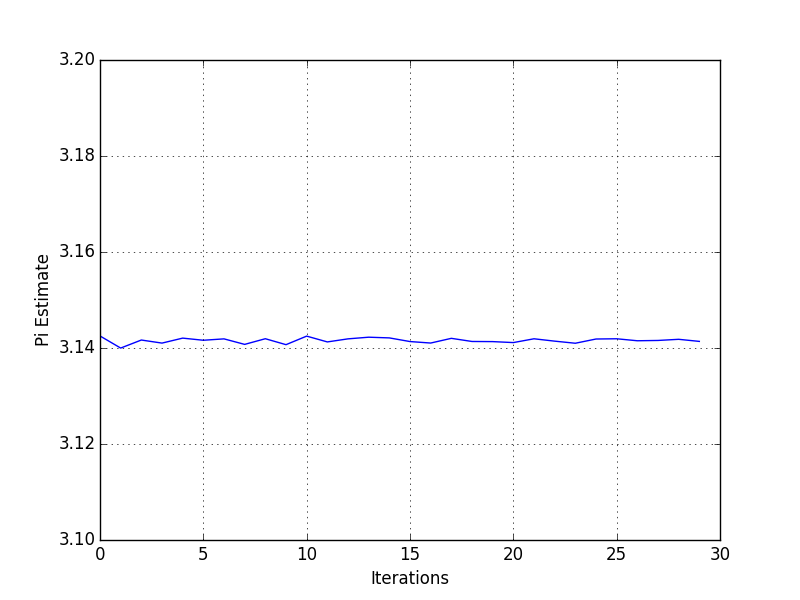
\includegraphics[scale=0.80]{pi_est.png}
    \caption{Estimate of the values of $\pi$}
	\label{fig:Y1}
\end{figure}

\begin{figure}[ht]
	\centering
    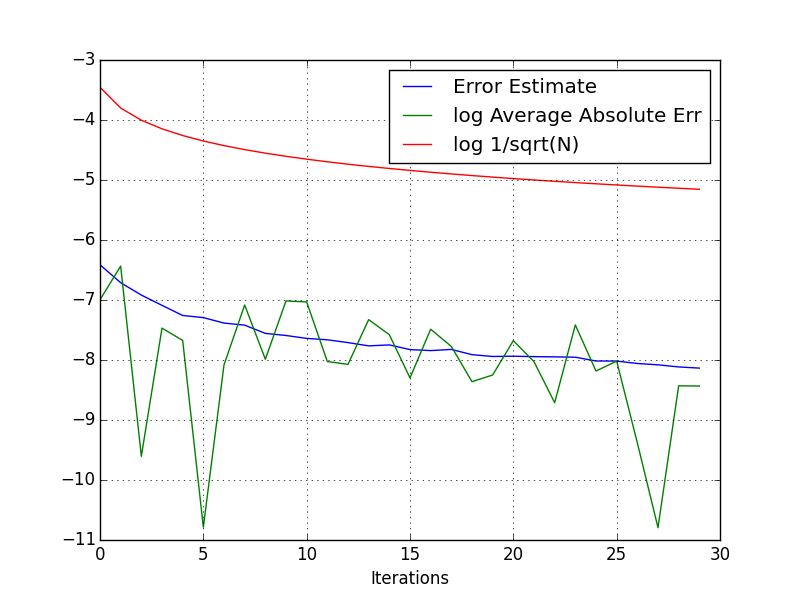
\includegraphics[scale=0.80]{err_est.png}
    \caption{change of error estimate and absolute error with increasing values of N. Here log($\frac{1}{\sqrt{N}}$) has been plotted for reference.}
	\label{fig:Y2}
\end{figure}

\begin{table}[ht]
\centering
\label{1b}
\begin{tabular}{|c|c|c|c|}
\hline
\textbf{N} & \textbf{Pi Estimate}&\textbf{$\log(\frac{\sigma}{\sqrt{N}}$)}&\textbf{Average Absolute Error} \\ \hline
1000 & 3.142508 & -6.41348792121 & -6.99620842209 \\
2000 & 3.139988 & -6.71147219026 & -6.43484712196 \\
3000 & 3.14166 & -6.91763448245 & -9.60566704811 \\
4000 & 3.141022 & -7.08901447367 & -7.46872748644 \\
5000 & 3.1420576 & -7.25796392872 & -7.67358928815 \\
6000 & 3.14161333333 & -7.2936121459 & -10.7863757461 \\
7000 & 3.14190171429 & -7.38430359819 & -8.0819742007 \\
8000 & 3.1407535 & -7.41917293679 & -7.08311631649 \\
9000 & 3.14193244444 & -7.55625404967 & -7.98718147024 \\
10000 & 3.1406948 & -7.59155617352 & -7.0155030864 \\
11000 & 3.14247527273 & -7.63964380553 & -7.03261724305 \\
12000 & 3.14126566667 & -7.66343122719 & -8.0255891238 \\
13000 & 3.14190461538 & -7.71002347021 & -8.07263114507 \\
14000 & 3.14225 & -7.7644752777 & -7.32730004188 \\
15000 & 3.142104 & -7.74859962632 & -7.57846409317 \\
16000 & 3.14134375 & -7.82647958467 & -8.29844327801 \\
17000 & 3.14103223529 & -7.8432896092 & -7.48682636454 \\
18000 & 3.14201311111 & -7.82393930635 & -7.77416807873 \\
19000 & 3.14135894737 & -7.91094478818 & -8.36144394036 \\
20000 & 3.1413314 & -7.94131111675 & -8.2500174438 \\
21000 & 3.14112952381 & -7.93669418525 & -7.67750235447 \\
22000 & 3.14191890909 & -7.94388132238 & -8.02783099513 \\
23000 & 3.141428 & -7.94778029614 & -8.71166425548 \\
24000 & 3.14099083333 & -7.95348895198 & -7.41555105294 \\
25000 & 3.14187184 & -8.01644609615 & -8.1836323316 \\
26000 & 3.141922 & -8.01782795101 & -8.01840168809 \\
27000 & 3.1415082963 & -8.05814633533 & -9.38044442293 \\
28000 & 3.14157214286 & -8.0804222317 & -10.7945422655 \\
29000 & 3.14181075862 & -8.11554628555 & -8.43053569888 \\
30000 & 3.14137533333 & -8.13521894018 & -8.43413656861 \\
\hline
\end{tabular}
\caption{Table of Values for the $\pi$ esimate using Monte Carlo Simulations.}
\end{table}
\textbf{What relation does the error estimate follow?}
\\It goes down as $\frac{1}{\sqrt{N}}$ with the number of iterations N. As can be seen in \ref{fig:Y2}
\\\textbf{What about the absolute error?}
\\The absolute error goes down approximately linearly.


The corresponding python code can be found at \ref{code:problem1b}
\clearpage
\section{Solution Q3}\label{prob3}
In this problem we are trying to Identify which meathod, Importance Sampling or Sample Mean method, we should choose for the task of identifying integrals given a function and its limits. To choose between them, we use each of the methods to perform a definite integral $\int_{1}^{2} (2x^{8}-1) dx$. After executing both the methods, we plot their respective absolute error with the analytically calculated exact integral value of 112.5555 We then state our conclusion below. 
\begin{figure}[ht]
	\centering
    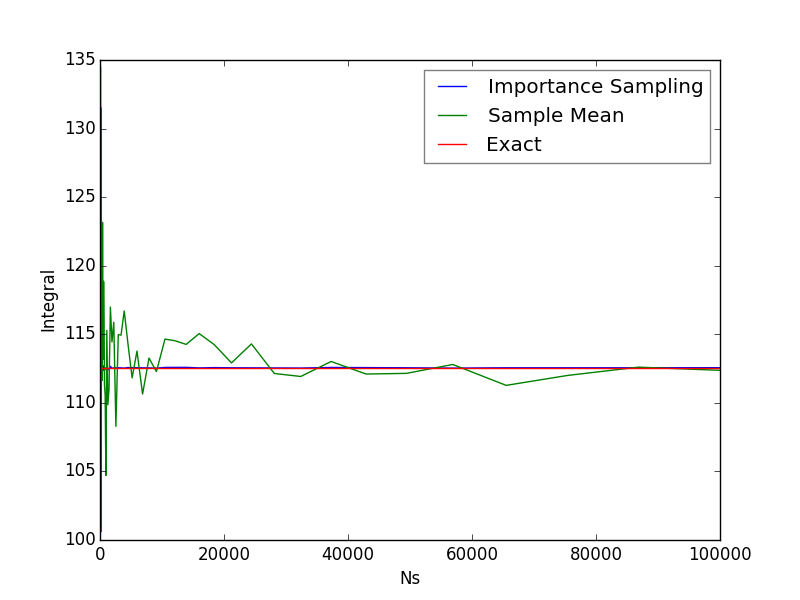
\includegraphics[scale=0.80]{Integrals.png}
    \caption{Value of Integral calculated using Importance sampling and Sample Mean method as a function of the Number of random samples. The exact value is plotted in Red for comparison.}
	\label{fig:errors}
\end{figure}


\begin{figure}[ht]
	\centering
    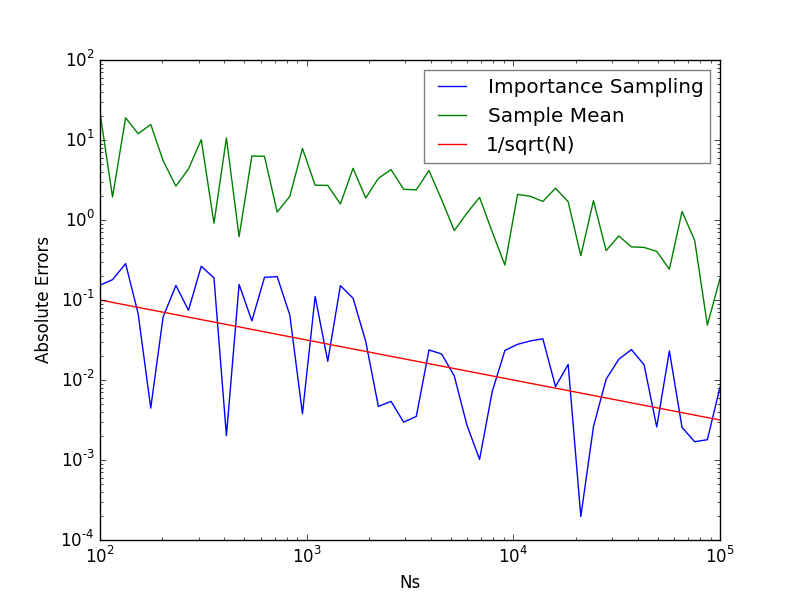
\includegraphics[scale=0.80]{Errors.png}
    \caption{Absolute errors of Integrals calculated using Importance sampling and Sample mean method, when compared to the actual analytic integral. The values have been plotted in the log scale}
	\label{fig:errors}
\end{figure}


\begin{table}[ht]
\centering
\label{table:1b}
\begin{tabular}{|c|c|c|c|c|}
\hline
\textbf{N} & \textbf{Imp samp est}&\textbf{Abs Err Imp Samp}&\textbf{Sample Mean Est}&\textbf{Abs Err Sample Mean} \\ \hline
    100 & 112.817602096 & 0.262046540193 & 97.6200018902 & 14.9355536653 \\
    115 & 112.790934035 & 0.235378479495 & 110.387517365 & 2.1680381906 \\
    133 & 112.862782704 & 0.307227148659 & 124.198178589 & 11.6426230335 \\
    153 & 112.307040131 & 0.248515424259 & 116.378833157 & 3.8232776018 \\
    176 & 112.570447868 & 0.01489231282 & 115.172083115 & 2.6165275593 \\
    202 & 112.807401366 & 0.251845810884 & 108.951693299 & 3.60386225665 \\
    233 & 112.605799413 & 0.0502438576779 & 106.077739978 & 6.47781557707 \\
    268 & 112.727453517 & 0.171897961599 & 128.263364923 & 15.7078093672 \\
   ...&...&...&...&...\\
    720 & 112.425498173 & 0.130057382117 & 104.21269517 & 8.3428603851 \\
    7906 & 112.591896217 & 0.0363406610969 & 111.628379791 & 0.927175764348 \\
    9103 & 112.593672719 & 0.0381171632268 & 115.933335012 & 3.37777945607 \\
    10481 & 112.593388655 & 0.0378330998116 & 110.255123721 & 2.30043183446 \\
    12068 & 112.544424017 & 0.0111315383437 & 112.60262766 & 0.0470721040552 \\
    13895 & 112.578383621 & 0.0228280654867 & 112.317530107 & 0.238025448329 \\
    15999 & 112.57870659 & 0.0231510344667 & 114.266579722 & 1.71102416604 \\
    18421 & 112.584252555 & 0.0286969996644 & 113.82109461 & 1.26553905427 \\
    21210 & 112.567439326 & 0.011883770476 & 111.959205762 & 0.596349793541 \\
    24421 & 112.525425965 & 0.0301295907316 & 113.264044066 & 0.708488510236 \\
    28118 & 112.565090954 & 0.00953539796538 & 113.32274423 & 0.767188674465 \\
    32375 & 112.543195441 & 0.0123601148601 & 111.961554588 & 0.594000967337 \\
    37276 & 112.56452844 & 0.00897288431986 & 113.132173579 & 0.576618023773 \\
    42919 & 112.553776654 & 0.00177890148414 & 112.70115021 & 0.145594654239 \\
    49417 & 112.553603269 & 0.00195228660451 & 112.926394176 & 0.370838620377 \\
    56899 & 112.549206334 & 0.006349221845 & 111.432828844 & 1.12272671195 \\
    65513 & 112.583406579 & 0.0278510230071 & 112.367194506 & 0.188361049716 \\
    75431 & 112.544776726 & 0.0107788296986 & 113.524978805 & 0.969423249651 \\
    86851 & 112.561721621 & 0.00616606549636 & 112.540220207 & 0.0153353481125 \\
    100000 & 112.555043138 & 0.000512417685144 & 112.505272248 & 0.0502833078437 \\
\hline
\end{tabular}
\caption{Table showing the values of $\int_{1}^{2} (2x^{8}-1) dx$ Estimated using Importance sampling method, its Absolute Error followed by the values using Sample Mean Method and then its Absolute Error in the last column.}
\end{table}
\textbf{Which method is better?}
It can be seen from the graph above and also from the table of values below, that the absolute error achieved by Importance sampling is much lower than that achieved by sample mean method. Hence \textbf{Importance Sampling} method is better. 
\\The corresponding python code can be found at \ref{code:problem3}
\clearpage
\section{Appendix A}\label{code:problem1b}
Python source code for \ref{prob1b}.
{\footnotesize
\begin{lstlisting}

from __future__ import division
import numpy as np
import pylab as pl

def mc_circle_np(n):
    '''
    We would be drawing random samples from -1 to 1
    '''
    inside = 0
    x = np.random.random(n)*2-1
    y = np.random.random(n)*2-1
    inside = np.sum((np.square(x,out=x) + np.square(y,out=y)) < 1)
    return 4 * (inside/n)

if __name__ == '__main__':
    n = 1000
    pi = 3.141592654
    pi_est = []
    err_est = []
    avg_abs_err = []
    start,end,step = 1000,31000,1000
    for N in xrange(start,end,step):
        pis = np.zeros(n)
        for i in xrange(1000):
            pis[i] = mc_circle_np(N)
        pi_est_m = np.mean(pis)
        pi_est.append(pi_est_m)
        err_est_m = np.log(np.std(pis)/np.sqrt(n)) #Because we always have n (=1000) estimates
        err_est.append(err_est_m)
        avg_abs_err_m = np.log(np.abs(pi_est_m - pi))
        avg_abs_err.append(avg_abs_err_m)
        print("{} & {} & {} & {} \\\\".format(N,pi_est_m,err_est_m,avg_abs_err_m))

    pl.plot(pi_est)
    pl.ylabel("Pi Estimate")
    pl.ylim((3.1,3.2))
    pl.xlabel("Iterations")
    pl.grid()
    pl.savefig("pi_est.png")

    pl.figure()
    pl.plot(err_est)
    pl.plot(avg_abs_err)
    pl.xlabel("Iterations")
    pl.legend(["Error Estimate","Average Absolute Err"])
    pl.grid()
    pl.savefig("err_est.png")
    pl.show()

\end{lstlisting}
}
\clearpage
\section{Appendix B}\label{code:problem3}
Python source code \ref{prob3}.
{\footnotesize
\begin{lstlisting}

from __future__ import division
import numpy as np
import pylab as pl

one_by_nine = 1/9.0
nine_by_511 = 9/511.0
def getIest_Imp(N):
    y = np.random.random(N)
    # Inverse function calculated manually
    x = np.power(511*y + 1, one_by_nine)
    f = 2*np.power(x,8) -1
    w = nine_by_511 * np.power(x,8) 
    Iest = np.mean(np.true_divide(f,w))
    return Iest

def getIest_Sm(N):
    # b = 2 and a = 1 Hence b-a = 1 
    # which doesn't affect the integral 
    # has been omitted from the calculations
    x = np.random.random(N)+1 # shift the rnadom values between 1 and 2
    f = 2*np.power(x,8)-1
    Iest = np.mean(f)
    return Iest

if __name__ == '__main__':
    exact = 1013/9.0
    Iest_Imp = []
    absErr_Imp = []
    Iest_Sm = []
    absErr_Sm = []
    Ns = map(lambda x: int(round(x)), np.logspace(2, 5, 50))
    for N in Ns:
        estImp = getIest_Imp(N)
        Iest_Imp.append(estImp)
        errImp = abs(exact-estImp)
        absErr_Imp.append(errImp)

        estSm = getIest_Sm(N)
        Iest_Sm.append(estSm)
        errSm = abs(exact-estSm)
        absErr_Sm.append(errSm)

        print "{} & {} & {} & {} & {} \\\\".format(N,estImp,errImp,estSm,errSm)

    pl.loglog(Ns,absErr_Imp,label="Importance Sampling")
    pl.loglog(Ns,absErr_Sm,label="Sample Mean")
    pl.loglog(Ns,map(lambda x:1/(x**0.5),Ns),label="1/sqrt(N)")
    pl.legend(framealpha=0.5)
    pl.xlabel("Ns")
    pl.ylabel("Absolute Errors")

    pl.savefig("Errors.png")
    pl.show()
\end{lstlisting}
}
\end{document}

   

